\documentclass{standalone}
\usepackage{tikz}
\usepackage{ctex,siunitx}
\setCJKmainfont{Noto Serif CJK SC}
\usepackage{tkz-euclide}
\usepackage{amsmath}
\usetikzlibrary{patterns, calc}
\usetikzlibrary {decorations.pathmorphing, decorations.pathreplacing, decorations.shapes,}
\begin{document}
\small
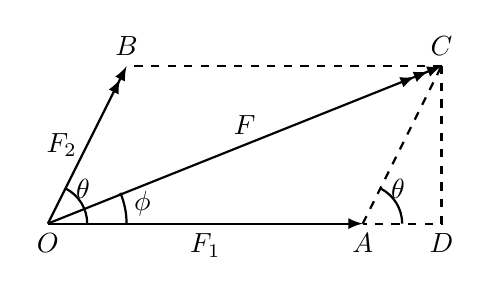
\begin{tikzpicture}[>=latex, thick,scale=1]
  % \useasboundingbox(-1,-0.75)rectangle(3.7,1.4);
  \draw [->](0,0)node[below] {$O$}--node[below] {$F_1$} (4,0)node[below] {$A$} ;
  \draw [->>](0,0)--node[left] {$F_2$}(1,2) node[above] {$B$};
  \draw [dashed](5,2)--(1,2);
  \draw [dashed](4,0)--(5,2)node[above] {$C$};
  \draw [->>>](0,0)--node[above] {$F$}(5,2) ;
  \draw [dashed](5,2)--(5,0) node[below] {$D$}--(4,0);
  \draw (.5,0) arc (0:63:.5) node[right] {$\theta$};
  \draw (1,0) arc (0:23:1);
  \draw (4.5,0) arc (0:63:.5) node[right] {$\theta$};
  \node at (1.2,.25) {$\phi$};
\end{tikzpicture}
\end{document}